\documentclass{../exercisesheet}

\title{Datenkommunikation und Informationssysteme, Übung 1}
\author{
    Domenic Quirl \\ 354437
    \and
    Julian Schakib \\ 353889
    \and 
    Daniel Schleiz \\ 356092
}

\renewcommand{\Exercise}{Aufgabe}
\date{Übungsgruppe 14}

\begin{document}
\maketitle
\pointtable

\begin{exercise}{3}
	Als \textit{Daten} bezeichnet man die Darstellung von einem Sachverhalt in einer definierten Form, sodass diese für die Kommunikation und technische Verarbeitung bereit sind.
	Die \textit{Information} ist dann die aus der Interpretation der Daten gewonnene Bedeutung, die ein Mensch oder eine Anwendung den Daten zuordnen kann. Unter \textit{Signalen}
	versteht man die physikalische Repräsentation von Daten, in welcher diese tatsächlich übertragen werden. \par
	Bezogen auf die in der Aufgabenstellung genannte Situation könnte man die Buchstaben auf dem Aushang als Daten interpretieren, welche den Text darstellen. Der Mensch,
	welcher diese Daten mithilfe von Sprache bzw. Grammatik interpretieren kann, zieht daraus die Information, dass er das Gericht Currywurstsuppe, welches als Tellergericht
	klassifiziert wird, zum Preis von 1,80 Euro erhalten kann. er Mensch nimmt diese Daten als optisches Signal in Form von Lichtreflektion wahr.\\
\end{exercise}

\begin{exercise}{5}
	\begin{subexercise}
		
	\end{subexercise}

	\begin{subexercise}
		  
	\end{subexercise}
\end{exercise}


\begin{exercise}{2}
	\begin{subexercise} \texttt{CONNECT.Request}\\
		Dieses Dienstprimitiv lässt sich mit der realen Aktion identifizieren, dass einer der Insassen einen Notruf absetzt und damit eine Verbindung aufbauen möchte. Der
		Insasse ruft also das Primitiv auf, das Pannenauto verarbeitet es.
	\end{subexercise}

	\begin{subexercise} \texttt{DATA.Indication}\\
		Dies lässt sich mit dem Ereignis, dass Gesprächsdaten vom Insassen angekommen sind, identifizieren. Dabei ruft das Leitstellensystem das Dienstprimitiv auf und
		ein Disponent verarbeitet es.
	\end{subexercise}

	\begin{subexercise} \texttt{DISCONNECT.Request}\\
		Das Drücken des Auflegen-Knopfs während eines Notrufs definiert dieses Dienstprimitiv. Es wird vom Insassen aufgerufen und vom Pannenauto verarbeitet.
	\end{subexercise}

	\begin{subexercise} \texttt{PROVIDERABORT.Indication}\\
		Dieses Dienstprimitiv wird beispielsweise aufgerufen, falls mitten im Notruf unerwarteterweise die Verbindung verloren geht. Es wird aufgerufen vom Pannenauto
		bzw. Leitstellensystem und verarbeitet vom Insassen bzw. Disponenten.
	\end{subexercise}
\end{exercise}

\begin{exercise}{1.5}
	Man könnte dies realisieren, indem der unbestätigte Dienst selbst wiederum im Sinne eines Schichtenmodells einen bestätigten Dienst für die Zustellung verwendet und die
	Übertragung so lange wiederholt, bis er die Confirmation erhalten hat. Eine Confirmation an den Dienstnutzer vom unbestätigten Dienst wird nicht gegeben, die Zustellung
	ist aber garantiert.\\
\end{exercise}

\begin{exercise}{3.5}
	\begin{subexercise}
		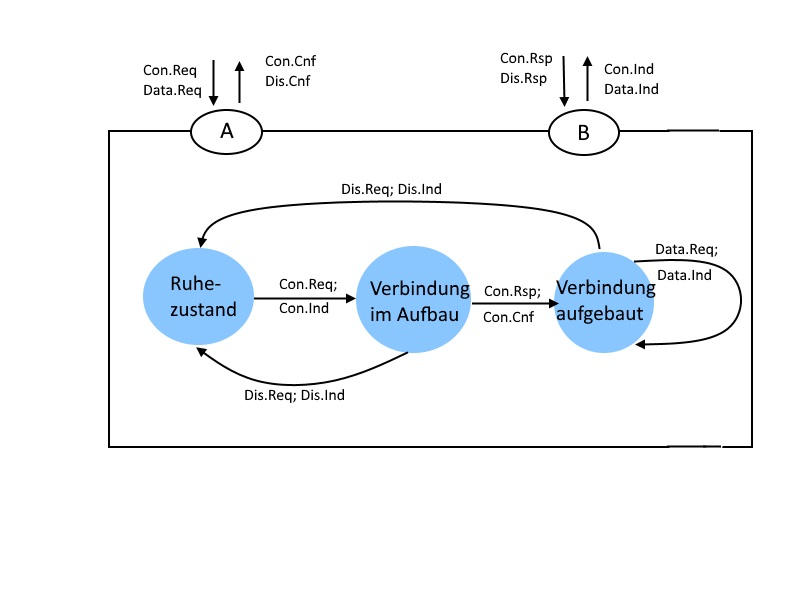
\includegraphics[scale=0.7]{1_5a.jpg}
	\end{subexercise}

	\begin{subexercise}
		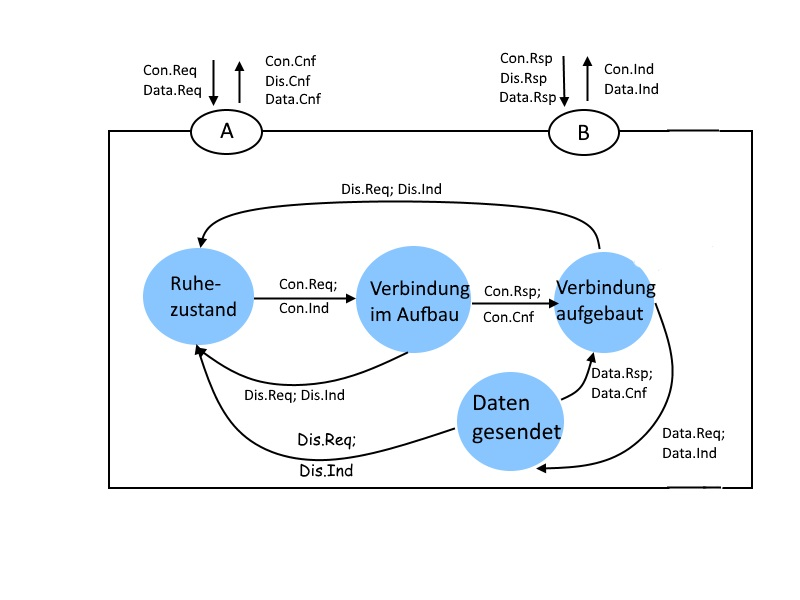
\includegraphics[scale=0.7]{1_5b.jpg}
	\end{subexercise}
\end{exercise}

\end{document}
